\documentclass[aspectratio=169]{beamer}

\title[Short Title]{
    ECE 555 Group Presentation
}
\author{
	% \tiny
	Igor Semyonov
	\and Jordan Carnes
	\and Robert Laverne Griffin
}
\institute{
    George Macon University, Department of Electrical and Computer Engineering
}

\usepackage{lmodern}
\usepackage[T1]{fontenc}

\usepackage{fix-cm}

%\usetheme{Berkeley}
% \usetheme{PaloAlto}
\usetheme{moloch}
\usecolortheme{albatross}

\usepackage{fancyvrb}

\logo{
	
\includegraphics[scale=0.1]{logo-gmu-ece.png }
}

\titlegraphic{
	
\includegraphics[scale=0.2]{./logo-gmu-ece.png}
}

\usepackage{graphicx}
\graphicspath{ {../figures/} }
\usepackage{float}
\usepackage{subcaption}

\setbeamercolor{normal text}{fg=white,bg=black!90}
\setbeamercolor{structure}{fg=white}

\setbeamercolor{alerted text}{fg=red!85!black}

\setbeamercolor{item projected}{use=item,fg=black,bg=item.fg!35}

\setbeamercolor*{palette primary}{use=structure,fg=structure.fg}
\setbeamercolor*{palette secondary}{use=structure,fg=structure.fg!95!black}
\setbeamercolor*{palette tertiary}{use=structure,fg=structure.fg!90!black}
\setbeamercolor*{palette quaternary}{use=structure,fg=structure.fg!95!black,bg=black!80}

\setbeamercolor*{framesubtitle}{fg=white}

\setbeamercolor*{block title}{parent=structure,bg=black!60}
\setbeamercolor*{block body}{fg=black,bg=black!10}
\setbeamercolor*{block title alerted}{parent=alerted text,bg=black!15}
\setbeamercolor*{block title example}{parent=example text,bg=black!15}


%\usepackage{natbib}
% \usepackage{bibentry}

\usepackage[english]{babel}% Recommended
\usepackage{csquotes}% Recommended
\usepackage[
	backend=biber,
	style=authoryear
]{biblatex}
\addbibresource[]{./refs.bib}% Syntax for version >= 1.2
% fix missing small caps
\renewcommand\mkbibacro[1]{{\footnotesize\MakeUppercase{#1}}}

\usepackage{graphicx} % Allows including images
\usepackage{booktabs} % Allows the use of \toprule
\usepackage{multirow}


%page numbers in bottom right
\setbeamertemplate{sidebar right}{}
\setbeamertemplate{footline}{%
	\hfill\usebeamertemplate***{navigation symbols}
	\hspace{1cm}\insertframenumber{}/\inserttotalframenumber}

% math
\usepackage{amsmath,amsfonts,amssymb,mathrsfs,mathtools}
\DeclarePairedDelimiter\abs{\lvert}{\rvert}%
\DeclarePairedDelimiter\norm{\lVert}{\rVert}%
% Swap the definition of \abs* and \norm*, so that \abs
% and \norm resizes the size of the brackets, and the 
% starred version does not.
\makeatletter
\let\oldabs\abs
\def\abs{\@ifstar{\oldabs}{\oldabs*}}

\DeclareMathOperator{\re}{Re}
\DeclareMathOperator{\im}{Im}
%
\let\oldnorm\norm
\def\norm{\@ifstar{\oldnorm}{\oldnorm*}}
\makeatother

% references for equations
\makeatletter
\def\tagform@#1{\maketag@@@{\bfseries(\ignorespaces#1\unskip\@@italiccorr)}}
\renewcommand{\eqref}[1]{\textup{{\normalfont(\ref{#1}}\normalfont)}}
\makeatother



% not using this, but can be nice
\usepackage{shadow}     % this creates a shaded box; see \shabox below


\usepackage{outlines}
%\usepackage[margin=1.0in]{geometry}
\setbeamersize{text margin left=15mm,text margin right=15mm}

% \usepackage{xparse}

\usepackage{tabto}
\NumTabs{6}

\newcommand{\eq}[2]{
    \begin{equation}\label{#1}
        #2
    \end{equation}
}

\usepackage{xspace}
\newcommand{\latex}{\LaTeX\xspace}
\newcommand{\tex}{\TeX\xspace}

\newcommand{\R}{\mathbb{R}}
\newcommand{\Rn}[1][n]{\mathbb{R}^#1}
\NewDocumentCommand{\Rnp}{ O{n} O{p} }{\mathbb{R}^#1_#2}



% \usepackage{mdframed}
% % \mdfdefinestyle{tablestyle}{linewidth=2pt}
% % \newmdframedend{markedtable}
% \surroundwithmdframed[
% linecolor=red,
% backgroundcolor=black,
% font={\sffamily},fontcolor=red]
% ]{table}
% % \mdfdefinestyle{exampledefault}{linewidth=2pt}
% % \newtheorem{my_example}{EXAMPLE}[chapter]

\newcommand{\figref}[1]{Figure \ref{#1}}
\newcommand{\lstref}[1]{Listing \ref{#1}}
\newcommand{\tabref}[1]{Table \ref{#1}}

\usepackage{listings, listings-rust}
\usepackage[framemethod=TikZ]{mdframed}
\lstset
{
	language=Rust,
	basicstyle=\footnotesize,
	numbers=left,
	numberstyle=\tiny,
	stepnumber=1,
	showstringspaces=false,
	tabsize=1,
	breaklines=true,
	breakatwhitespace=false,
	xleftmargin=-8pt,
	frame=T,
}
\newcommand{\codefileNoFigure}[3]{
	\mdframed[roundcorner=5pt, backgroundcolor=blue!30]
	% \lstinputlisting[caption=\texttt{#1} {#2}, label=#3]{#1}
	\lstinputlisting[caption={#2}, label=#3]{#1}
	\endmdframed
}
\newcommand{\codefileRustNoFigure}[3]{
	\mdframed[roundcorner=5pt, backgroundcolor=blue!30]
	\lstinputlisting[
		language=Rust,
		caption={#2},
		label=#3
	]{#1}
	\endmdframed
}
\newcommand{\codefile}[3]{
	\begin{figure}[H]
		\codefileNoFigure{#1}{#2}{#3}
	\end{figure}
}


\begin{document}

\begin{frame}
	\vspace{-1.8cm}
	\titlepage
\end{frame}

\begin{frame}
	\frametitle{Why not Just Use C?}
	\framesubtitle{}

    \begin{columns}
        \begin{column}{0.4\textwidth}
            \begin{itemize}
                \item No safety
                \item Skill issues, leading to lack of safety
            \end{itemize}
        \end{column}
    \end{columns}
\end{frame}

\begin{frame}
	\frametitle{Why Rust}
	\framesubtitle{Type System}

	\begin{columns}
		\begin{column}{0.4\textwidth}
			\lstinputlisting[
				linerange=1-9,
				caption=Cats,
				frame=tblr,
				language=Rust
			]{./code-snippets-rs/src/cats.rs}
		\end{column}
		\begin{column}{0.5\textwidth}
			Impossible states can be encoded in the type system, which leads to compile time errors, instead of runtime checks.
			\lstinputlisting[
				linerange=14-17,
				caption=Unphysical (zombie) Cat,
				frame=tblr,
				language=Rust
			]{./code-snippets-rs/src/cats.rs}
		\end{column}
	\end{columns}
\end{frame}

\begin{frame}
	\frametitle{Why Rust}
	\framesubtitle{Type System}
	\begin{figure}[ht]
		\centering
		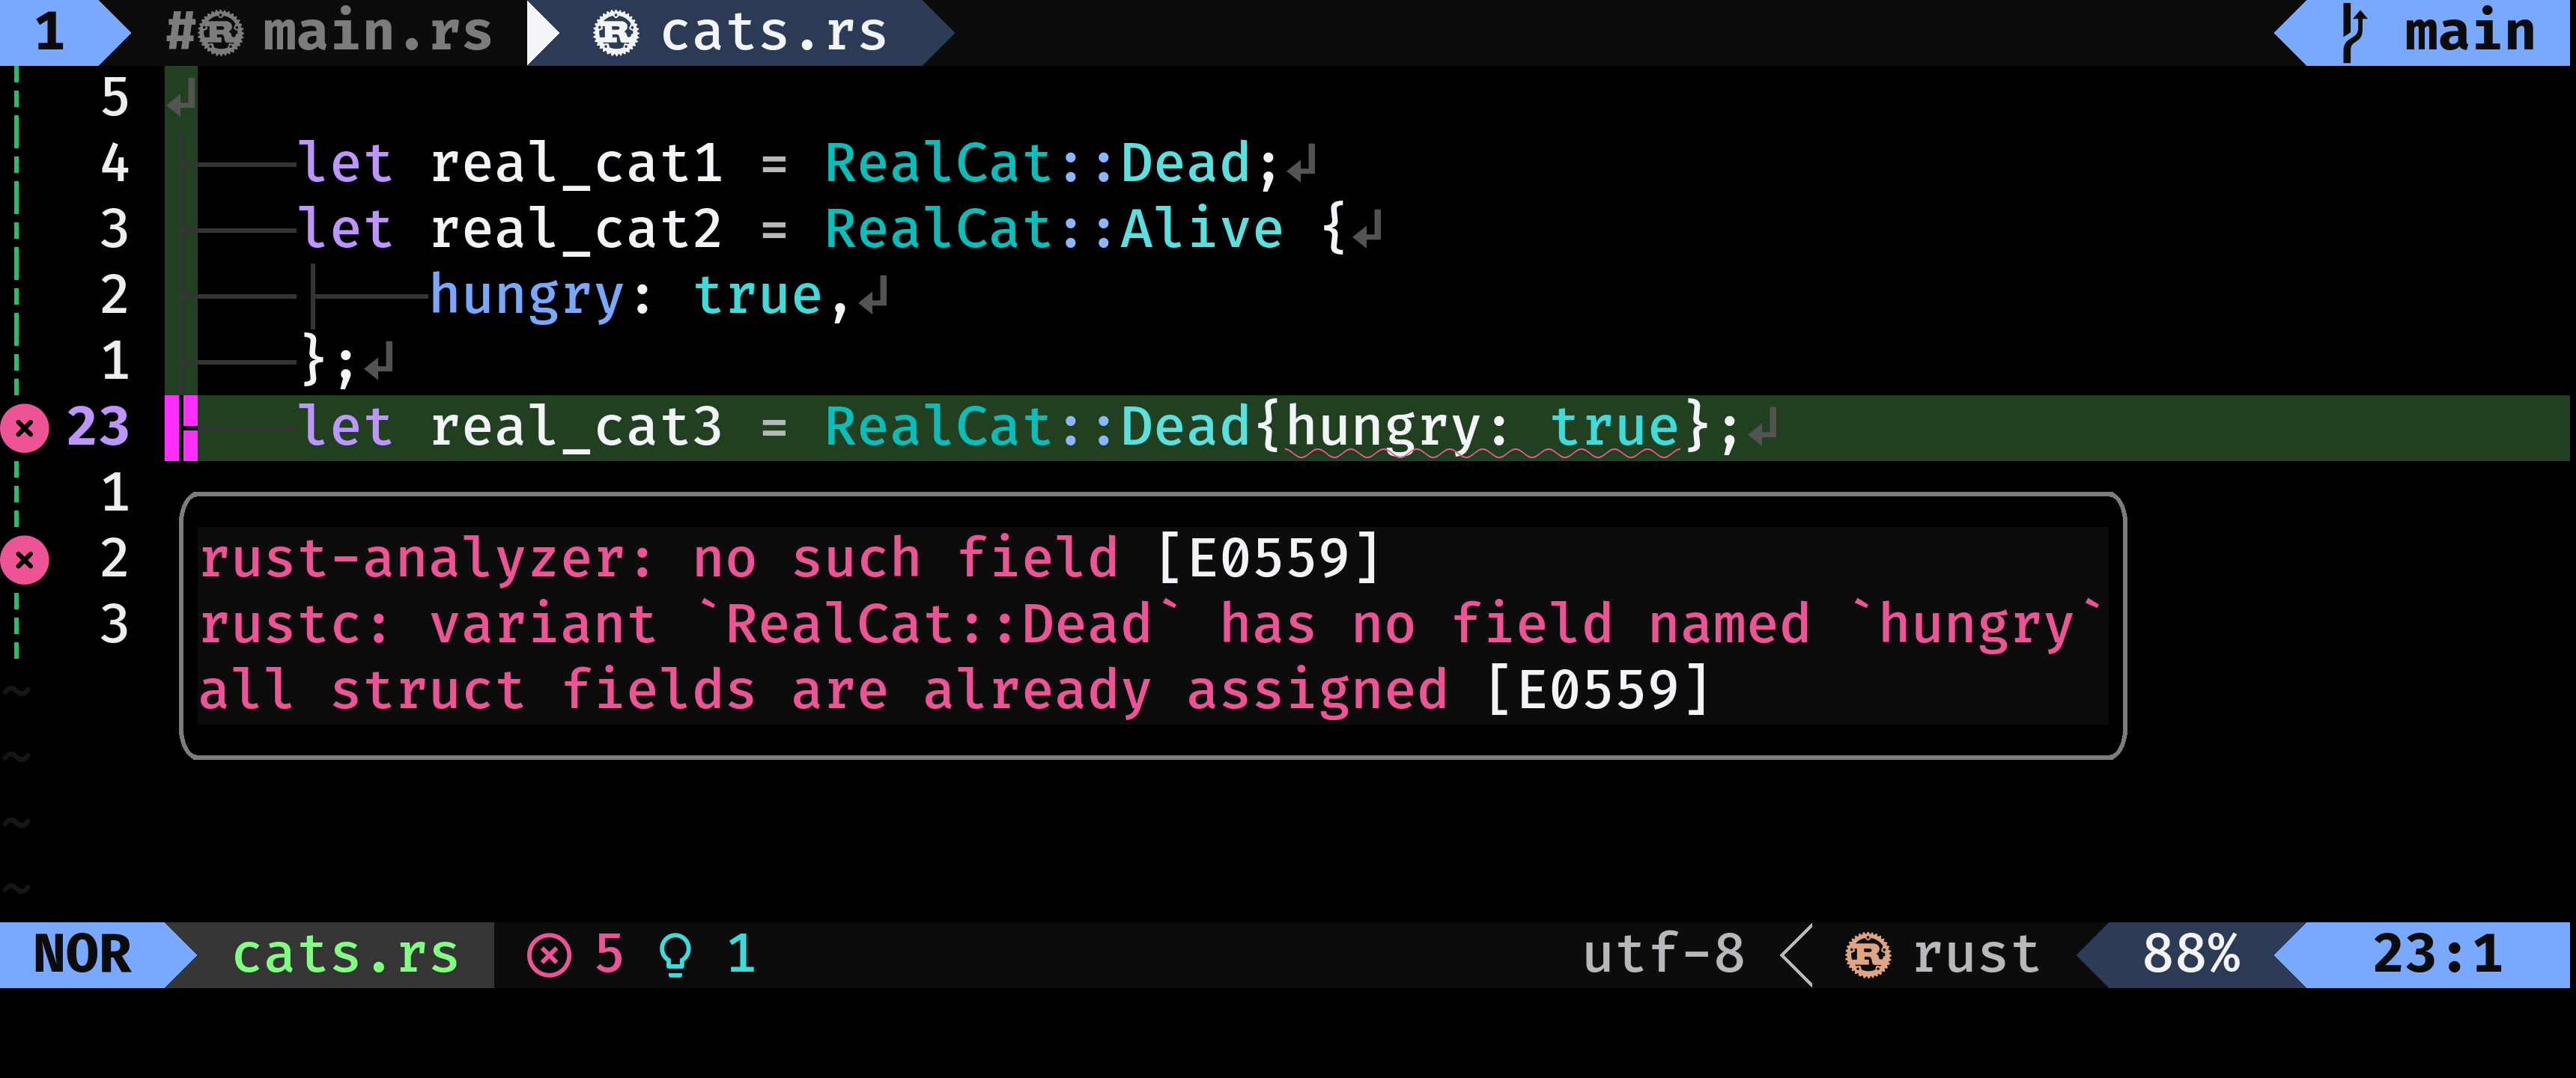
\includegraphics[width=\textwidth]{./figures/real-cat.png}
		\caption{Error when declaring an unrealistic cat}
	\end{figure}
\end{frame}

\begin{frame}
	\frametitle{Why Rust}
	\framesubtitle{Safety}

	\begin{columns}
		\begin{column}{0.4\textwidth}
			\begin{itemize}
				\item Result: Errors are values, i.e., no nidden control flow
				\item Functions that can fail return Result and this must be explicitly handled.
			\end{itemize}
		\end{column}
		\begin{column}{0.4\textwidth}
			\begin{itemize}
				\item No manual memory management
				\item Values are dropped once they go out of scope
			\end{itemize}
		\end{column}
	\end{columns}
\end{frame}

\begin{frame}
	\frametitle{Why Rust}
	\framesubtitle{Ergonomics}

	High level abstractions that enable multithreading without the error-prone approach of pthreads in C.
\end{frame}

\begin{frame}
	\frametitle{Why Rust}
	\framesubtitle{Single threaded bsort}
	\begin{columns}
		\begin{column}{ 0.5\textwidth }
			\lstinputlisting[
				linerange=6-7,
				caption=Single threaded bsort,
				frame=tblr,
				language=Rust
			]{./code-snippets-rs/src/project_1_example.rs}
		\end{column}
		\begin{column}{ 0.4\textwidth }
			\begin{itemize}
				\item \Verb|a| is a vector of numbers
				\item \Verb|chunks\_mut| slices the vector into non-overlapping slices of the given length
				\item \Verb|for\_each| iterates over the chunks, running the provided function with each chunk as the input.
			\end{itemize}
		\end{column}
	\end{columns}
\end{frame}

\begin{frame}
	\frametitle{Why Rust}
	\framesubtitle{Concurrency is easy while avoiding race conditions}
	\begin{columns}
		\begin{column}{ 0.5\textwidth }
			\lstinputlisting[
				linerange=2-4,
				caption=Example of easy parallelization,
				frame=tblr,
				language=Rust
			]{./code-snippets-rs/src/project_1_example.rs}
		\end{column}
		\begin{column}{ 0.4\textwidth }
			\begin{itemize}
				\item Chunks is known to split a vector into distinct slices
				\item Hence we can safely send each chunk to a different thread
			\end{itemize}
		\end{column}
	\end{columns}
\end{frame}

\begin{frame}
	\begin{figure}[ht]
		\centering
		\includegraphics[width=\textwidth]{./figures/project-1-plot.png}
		\caption{Preformacne results from bsort project. Note that the Rust reference sort is not plotted as it was under 1ms, compared to 8ms for the C qsort.}
	\end{figure}
\end{frame}

\begin{frame}
	\frametitle{Why Rust}
	\framesubtitle{Zero Cost Abstraction}

	All these features are provided at compile time and are optimized away when compiling so that they do not affect performance at run time.
\end{frame}

\begin{frame}
	\frametitle{Rust Ownership and Borrowing}
	\framesubtitle{Problems with shared memory access in Rust}

	\begin{columns}
		\begin{column}{0.5\textwidth}
			\begin{itemize}
				\item Ownership Rules\footnotemark
				      \begin{itemize}
					      \item Each value has an owner
					      \item There can only be one owner at a time
					      \item When the owner goes out of scope, the value will be dropped.
				      \end{itemize}
			\end{itemize}
		\end{column}
		\begin{column}{0.5\textwidth}
			\begin{itemize}
				\item Borrow Rules\footnotemark
				      \begin{itemize}
					      \item At any given time, you can have either one mutable reference or any number of immutable references.
					      \item References must always be valid.
				      \end{itemize}
			\end{itemize}
		\end{column}
	\end{columns}

	\vspace{1cm}
	C, and especially CUDA, style shared mutable memory access violates the ownership and borrow rules.

	At this time, we therefore need to use unsafe Rust when writing and calling GPU kernels.

	\footnotetext{ [Ch04-01]{rust-book}}
	\footcitetext[Ch04-02]{rust-book}
\end{frame}

\begin{frame}
	\frametitle{Rust and GPU Programming}
	\framesubtitle{Current options}

	\begin{itemize}
		\item Rust GPU for vendor agnostic GPU programming
		\item Rust CUDA for targeting NVIDIA GPUs and their specific libraries
		\item Vulkano
		\item wgpu
		\item Miniquad
		\item Sierra
		\item Glium
		\item Ash
		\item Erupt
	\end{itemize}

	We focused on the Rust CUDA crate, which is currently in active development.
\end{frame}

\begin{frame}
	\frametitle{What is a compiler?}
	\framesubtitle{Translation pipeline}

	\begin{columns}[T]
		\begin{column}{0.3\textwidth}
			Front End
			\begin{itemize}
				\item Lexical analysis: source → tokens (identifiers, literals, operators)
				\item Syntax \& semantic analysis: tokens → AST, type checking
				\item Emit language independent IR
			\end{itemize}
		\end{column}
		\begin{column}{0.4\textwidth}
			Optimization
			\begin{itemize}
				\item IR level passes: constant folding, dead code elimination, algebraic simplification
				\item Advanced transforms: function inlining, loop unrolling, vectorization
				\item Profile  or link time optimizations for extra performance
			\end{itemize}
		\end{column}
		\begin{column}{0.3\textwidth}
			Back End
			\begin{itemize}
				\item Lower optimized IR to machine instructions (instruction selection \& scheduling)
				\item Register allocation, calling‐convention handling
				\item Emit assembly or object code ready for linking
			\end{itemize}
		\end{column}
	\end{columns}
\end{frame}

\begin{frame}
	\frametitle{The problem LLVM solves}
	\framesubtitle{front ends \& back ends}

	\begin{columns}[T]
		\begin{column}{0.25\textwidth}
			Fragmented Toolchains
			\begin{itemize}
				\item Historically each language writes its own optimizer \& code generator
				\item Reinventing the same analyses over and over
			\end{itemize}
		\end{column}
		\begin{column}{0.25\textwidth}
			Reusable IR
			\begin{itemize}
				\item SSA based intermediate form shared by many languages
				\item Single place to build and maintain optimizations
			\end{itemize}
		\end{column}
		\begin{column}{0.25\textwidth}
			Multiple back ends
			\begin{itemize}
				\item Add support for x86, ARM, RISC V, NVIDIA GPUs, … by writing one backend
				\item All front ends instantly benefit from each new target
			\end{itemize}
		\end{column}
		\begin{column}{0.25\textwidth}
			Rapid language support
			\begin{itemize}
				\item New languages (Rust, Swift, Julia, etc.) get mature codegen “for free”
				\item Performance improvements flow to every user automatically
			\end{itemize}
		\end{column}
	\end{columns}
\end{frame}

\begin{frame}
	\frametitle{NVVM}
	\framesubtitle{NVIDIA’s LLVM based GPU IR}

	\begin{columns}[T]
		\begin{column}{0.4\textwidth}
			What is NVVM IR? \footnotemark
			\begin{itemize}
				\item A dialect of LLVM IR extended for CUDA style GPU programming
				\item Adds memory space qualifiers (global, shared, constant)
			\end{itemize}
		\end{column}
		\begin{column}{0.4\textwidth}
			Metadata \& intrinsics
			\begin{itemize}
				\item Thread/block IDs and barriers (llvm.nvvm.barrier0)
				\item Marks kernel entry points and resource usage requirements
			\end{itemize}
		\end{column}
	\end{columns}
	\footcitetext{supercomputing}
\end{frame}

\begin{frame}
	\frametitle{NVVM}
	\framesubtitle{NVIDIA’s LLVM based GPU IR (continued)}

	\begin{columns}[T]
		\begin{column}{0.4\textwidth}
			Toolchain flow
			\begin{enumerate}
				\item Front end emits .nvvm.bc bitcode file
				\item NVVM compiler (libnvvm) lowers IR to PTX assembly
				\item PTX → CUBIN or JIT compiled by CUDA driver at runtime
			\end{enumerate}
		\end{column}
		\begin{column}{0.4\textwidth}
			Why use NVVM?
			\begin{itemize}
				\item Reuse LLVM’s optimizer on device code
				\item Keep host and GPU code in one common IR for easier shared analysis
			\end{itemize}
		\end{column}
	\end{columns}
\end{frame}

\begin{frame}
	\frametitle{Rust CUDA and NVVM}
	\framesubtitle{How the pieces fit}

	\begin{columns}[T]
		\begin{column}{0.4\textwidth}
			Cargo \& rustc target \footnotemark
			\begin{itemize}
				\item Compile kernels with --target=nvptx64-nvidia-cuda
				\item Separate build profiles for host (x86\_64) and device (PTX)
			\end{itemize}
		\end{column}
		\begin{column}{0.4\textwidth}
			LLVM IR generation
			\begin{itemize}
				\item Annotate GPU functions with \texttt{\#[kernel]} or \texttt{extern "ptx-kernel"}
				\item rustc emits NVVM compatible IR carrying thread/block metadata
			\end{itemize}
		\end{column}
	\end{columns}
	\footcitetext{rust-for-gpu}
\end{frame}

\begin{frame}
	\frametitle{Rust CUDA and NVVM}
	\framesubtitle{How the pieces fit (continued)}

	\begin{columns}[T]
		\begin{column}{0.4\textwidth}
			PTX emission
			\begin{itemize}
				\item Build script (\texttt{build.rs}) or \Verb|nvptx-link| plugin calls into \Verb|libnvvm|
				\item Produces \Verb|.ptx| files you bundle into your binary or load at runtime
			\end{itemize}
		\end{column}
		\begin{column}{0.4\textwidth}
			Runtime loading \& launch
			\begin{itemize}
				\item Use the \Verb|rustacuda| crate (or raw CUDA Driver API) to load modules
				\item Launch kernels inside \Verb|unsafe| blocks, mirroring C/CUDA calls
			\end{itemize}
		\end{column}
	\end{columns}
\end{frame}

\section{Demo Implementation}

\begin{frame}
	\frametitle{Fractals}
	\framesubtitle{Mandelbrot and Burning Ship}
	$c \in \mathbb{C}$ is in the mandelbrot set if the sequence $\{z_n\}$ converges.

	\begin{equation*}
		z_{n+1} := z_n^2 + c \hspace{1cm} z_0 = 0
	\end{equation*}

	The Burning Ship fractal is defined similarly but the sequence is

	\begin{equation*}
		z_{n+1} := (\abs{\re(z_n)} + \abs{\im(z_n)}i)^2 + c \hspace{1cm} z_0 = 0
	\end{equation*}
\end{frame}

\begin{frame}
	\frametitle{Mandelbrot Kernel}
	% \framesubtitle{Mandelbrot and Burning Ship}
	\begin{columns}
		\begin{column}{0.5\textwidth}
			\lstinputlisting[
				linerange=48-70,
				basicstyle=\tiny,
				% caption=,
				frame=tblr,
				language=Rust
			]{../code/gpu/fractals/src/lib.rs}
		\end{column}
		\begin{column}{0.45\textwidth}
			\lstinputlisting[
				linerange=72-89,
				firstnumber=24,
				basicstyle=\tiny,
				% caption=,
				frame=tblr,
				language=Rust
			]{../code/gpu/fractals/src/lib.rs}
		\end{column}
	\end{columns}
\end{frame}

\begin{frame}
	\frametitle{Launching the Kernel}
	% \framesubtitle{Mandelbrot and Burning Ship}
	\begin{columns}
		\begin{column}{0.55\textwidth}
			\lstinputlisting[
				linerange=205-220,
				basicstyle=\tiny,
				% caption=,
				frame=tblr,
				language=Rust
			]{../code/cpu/fractals/src/main.rs}
		\end{column}
		\begin{column}{0.3\textwidth}
			\begin{itemize}
				\item Fiarly similar to launching a kernel in C.
				\item Must be used inside an \Verb|unsafe| block since the kernel itself is an unsafe function.
			\end{itemize}
		\end{column}
	\end{columns}
\end{frame}

\begin{frame}
	\frametitle{Output Image}
	\begin{figure}[H]
		\centering
		
\includegraphics[width=\textwidth]{./figures/mandelbrot.png}
	\end{figure}
\end{frame}

\begin{frame}
	\frametitle{Fractals}
	% \framesubtitle{Timing Results for 1 frame on CPU and GPU}

	\begin{columns}
		\begin{column}{0.5\textwidth}
			\begin{table}[ht]
                \centering
                \caption{Timing results for several approaches of producing the fractals}
				\begin{tabular}{l r}
					\toprule
					Method                & Time (ms) \\
					\midrule
					CPU create point grid & 175.357   \\
					GPU using CPU points  & 0.552     \\
					CPU using rayon       & 143.647   \\
					\midrule
					GPU f32               & 0.453     \\
					GPU f64               & 12.272    \\
					\bottomrule
				\end{tabular}
			\end{table}
		\end{column}
	\end{columns}
\end{frame}

\begin{frame}
	\frametitle{Fractals}
	% \framesubtitle{Live Demo}

	\centering
	\huge Live Demo
\end{frame}

\printbibliography

\end{document}
